% !TEX root = ../../defense.tex

\section{Shape Reconstruction}
\begin{frame}{Asteroid Shape Modeling}
    \begin{itemize}
        \item<1-> Ground radar used to compute the 3D shape of the asteroid
        \begin{itemize}
            \item Computationally intensive estimation algorithm completed on the ground 
            \item The result is still coarse and only an approximation solution
            \item Not accurate enough for low altitude or landing operations
        \end{itemize}
    \item<2-> Estimating the asteroid shape is the first step of any mission
    \begin{itemize}
        \item Months or years are devoted solely to mapping the surface
        \item Laser ranging used to accurately measure relative distance 
        \item All data is sent to the ground for processing (time and manpower intensive)
    \end{itemize}
    \end{itemize}
    
    \onslide<3->{
        \begin{block}{}
            \begin{center}
                Real-time on board shape estimation
            \end{center}
        \end{block}
    }
\end{frame}

\section[Problem Statement]{Math Background}
\begin{frame}{Problem Statement}
\begin{enumerate}
    \item<1-> Compute the surface shape from range measurements
        \begin{itemize}
            \item Real time and incrementally build the shape
        \end{itemize}
    \item<2-> Utilize shape model in dynamics and controller
        \begin{itemize}
            \item Coupled equations of motion 
            \item Nonlinear controller for maneuvering and landing
        \end{itemize}
    \item<3-> Autonomously navigate around asteroid 
        \begin{itemize}
            \item Locate areas of poor knowledge for measurement
            \item Avoid obstacles or hazards
        \end{itemize}
\end{enumerate}
\end{frame}

\begin{frame}{LIDAR Measurements }
    \begin{itemize}
        \item<1-> Laser pulse used to measure relative distance to surface
        \item<1-> Accurate timing gives the round trip time of flight
            \begin{align*}
                d = \frac{\Delta t}{2 c}
            \end{align*}
    \end{itemize}
     
    \begin{center}
        \only<1>{
            \resizebox{!}{0.6\textheight}{
                \tikzsetnextfilename{laser_range_finder}
\begin{tikzpicture}[
    block/.style={rectangle,thick,
        draw=blue!50,
        fill=blue!20, 
        rounded corners, 
        text centered, 
        minimum height = 3em, 
        minimum width=6em},
        on grid=false,
        node distance=3em,
        auto,
    ]

    \node [block] (detector) {Detector};
    \node [block, below = of detector] (amplifier) {Amplifier};
    \node [block, right = of amplifier] (transmitter) {Transmitter};
    \node [block, below = of $(amplifier)!0.5!(transmitter)$] (timer)  {Clock};
    \node [block, right = of detector] (beamsplitter) {Optics};
    \node [block, right = of beamsplitter] (target) {Target};
    
    \node [below = of timer] (system) {};

    \draw[-Latex] (amplifier) |- node[left] {\scriptsize Stop pulse}  (timer.west);
    \draw[-Latex] (transmitter.south) |- node[right] {\scriptsize Start pulse} (timer.east);
    \draw[-Latex] (detector.south) -- (amplifier.north);

    \draw[-Latex] (transmitter.north) -- (beamsplitter.south);
    \draw[->,decorate,
        decoration={snake,amplitude=.4mm,segment length=2mm,post length=1mm}] (beamsplitter.350) -- (target.190);
    \draw[->,decorate,
        decoration={snake,amplitude=.4mm,segment length=2mm,post length=1mm}] (target.170) -- (beamsplitter.10);

    \draw[-Latex] (beamsplitter) -- (detector);
    \draw[-Latex] (timer) -- node[left] {\scriptsize $\Delta t$} (system);
\end{tikzpicture}

            }
        }
        \only<2>{
            \tikzsetnextfilename{frustrum}
\begin{tikzpicture}[scale=1.7]

    \pgfmathsetmacro{\posalongpath}{0.37}
    \pgfmathsetmacro{\distance}{6};
    \pgfmathsetmacro{\nearplane}{0.37};
    \pgfmathsetmacro{\hfov}{15};
    \pgfmathsetmacro{\wfov}{15};
    \pgfmathsetmacro{\H}{\distance*tan(\hfov/2)};
    \pgfmathsetmacro{\W}{\distance*tan(\wfov/2)};
    \pgfmathsetmacro{\dlength}{1};

    \pgfmathsetmacro{\conex}{1};
    \pgfmathsetmacro{\coney}{0};
    \pgfmathsetmacro{\conez}{0};

    \pgfmathsetmacro{\ctwox}{0};
    \pgfmathsetmacro{\ctwoy}{1};
    \pgfmathsetmacro{\ctwoz}{0};

    \pgfmathsetmacro{\cthreex}{0};
    \pgfmathsetmacro{\cthreey}{0};
    \pgfmathsetmacro{\cthreez}{1};
    
    \coordinate (V) at (0,0,0);
    \coordinate (A) at ($ (\distance * \conex, \distance * \coney, \distance * \conez) + (-\W * \ctwox, -\W * \ctwoy, -\W * \ctwoz) + ( \H * \cthreex, \H * \cthreey, \H * \cthreez) $);
    \coordinate (B) at ($ (\distance * \conex, \distance * \coney, \distance * \conez) + (\W * \ctwox, \W * \ctwoy, \W * \ctwoz) + ( \H * \cthreex, \H * \cthreey, \H * \cthreez) $);
    \coordinate (C) at ($ (\distance * \conex, \distance * \coney, \distance * \conez) + (\W * \ctwox, \W * \ctwoy, \W * \ctwoz) + ( -\H * \cthreex, -\H * \cthreey, -\H * \cthreez) $);
    \coordinate (D) at ($ (\distance * \conex, \distance * \coney, \distance * \conez) + (-\W * \ctwox, -\W * \ctwoy, -\W * \ctwoz) + ( -\H * \cthreex, -\H * \cthreey, -\H * \cthreez) $);

    \coordinate (m1) at ($ (V) + (\dlength * \conex, \dlength * \coney, \dlength * \ctwoz )$);
    \coordinate (m2) at ($ (V) - (\dlength * \conex, \dlength * \coney, \dlength * \ctwoz )$);

    \path (A) -- (V) coordinate[pos=\posalongpath] (A-V);
    \path (B) -- (V) coordinate[pos=\posalongpath] (B-V);
    \path (C) -- (V) coordinate[pos=\posalongpath] (C-V);
    \path (D) -- (V) coordinate[pos=\posalongpath] (D-V);
    
    % labels of points
    \node[below] at (A) {$A$};
    \node[above] at (B) {$B$};
    \node[above] at (C) {$C$};
    \node[right] at (D) {$D$};

    \draw[red!50!black, dashed] (V) -- (A-V) (V) -- (B-V) (V) -- (C-V) (V) -- (D-V);
    % \draw[red!50!black] (A) -- (A-V) (B) -- (B-V) (C) -- (C-V) (D) -- (D-V);
    \draw[red!50!black, -Latex] (A-V) -- (A);
    \draw[red!50!black, -Latex] (B-V) -- (B);
    \draw[red!50!black, -Latex] (C-V) -- (C);
    \draw[red!50!black, -Latex] (D-V) -- (D);
    \fill[red,opacity=0.5,draw=red!80!black,thick] (A) -- (B) -- (C) -- (D) -- cycle;
    \fill[blue,opacity=0.5,draw=blue!80!black,thick] (A-V) -- (B-V) -- (C-V) -- (D-V) -- cycle; 
    
    \draw[blue!50!black, ultra thick] (m1) -- (m2);
    \shade[ball color=blue] (m1) circle (0.2);
    \shade[ball color=blue] (m2) circle (0.2);

\end{tikzpicture}

        }
        \only<3>{
            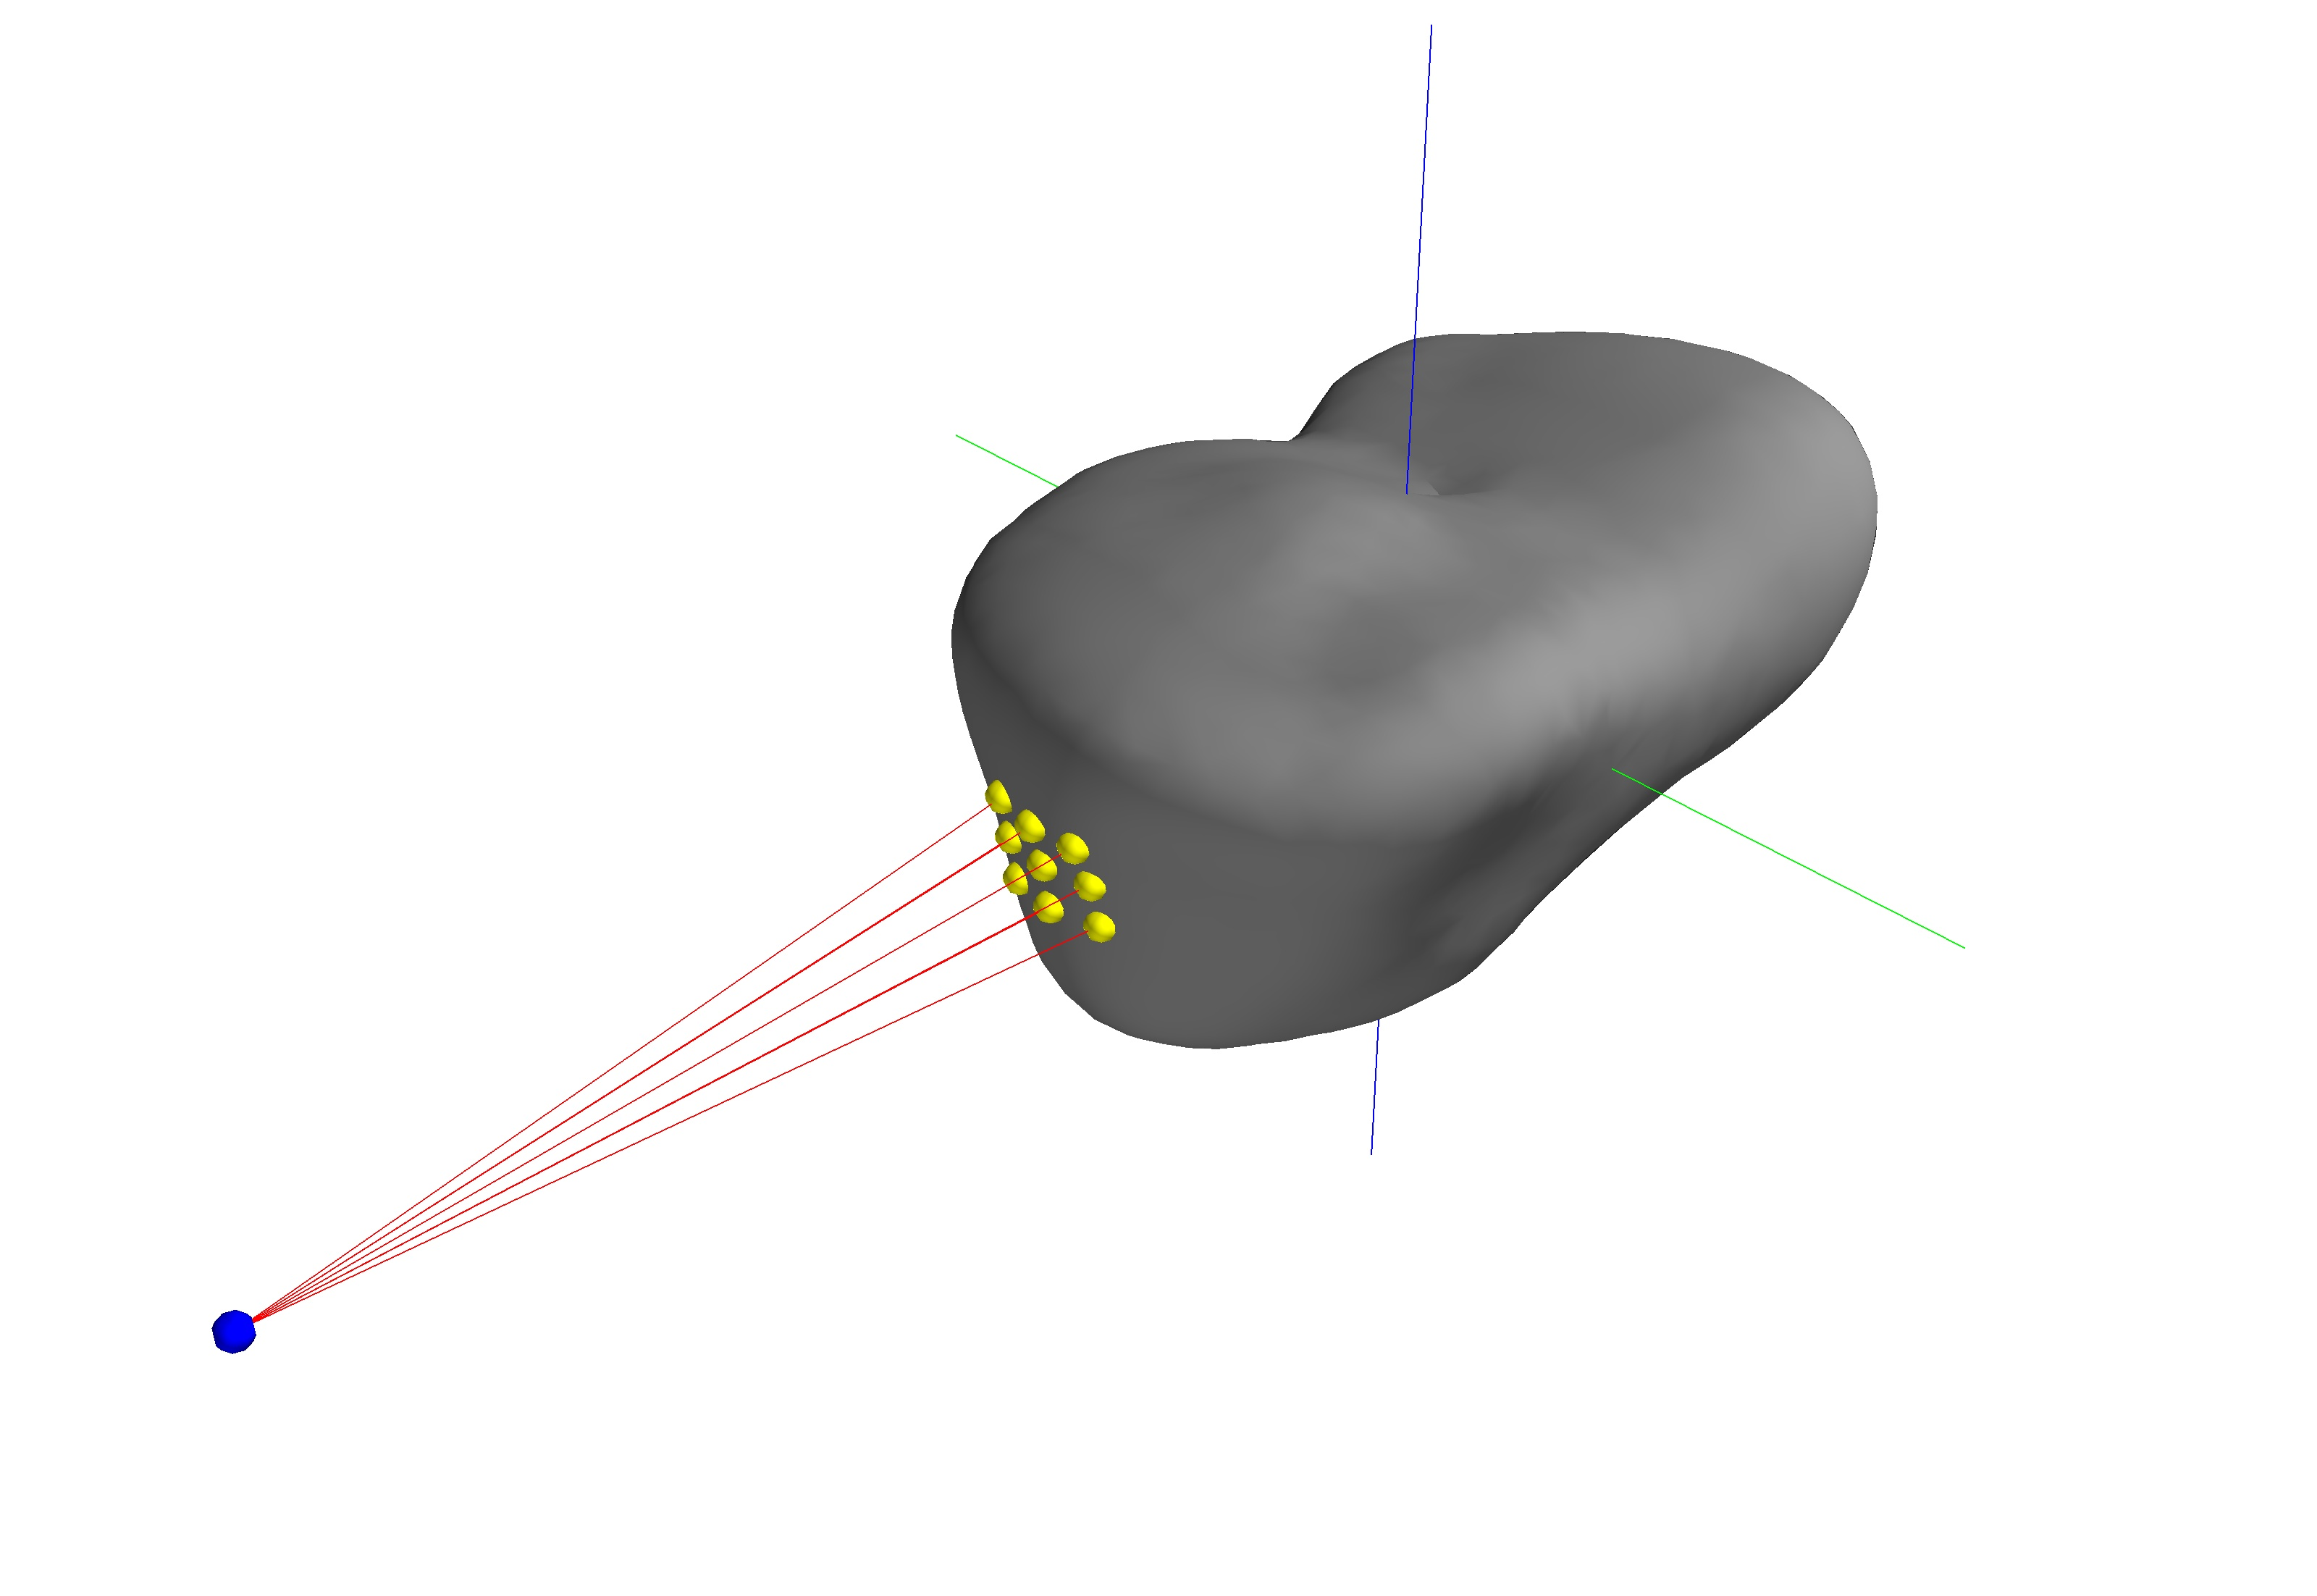
\includegraphics[width=0.75\textwidth,height=0.7\textheight,keepaspectratio]{figures/2018_SSPI/castalia_raycasting_plot.jpg}
        }
    \end{center}
\end{frame}

\begin{frame}{Bayesian Shape Reconstruction}
    \begin{itemize}
        \item<1-> Framework for combining prior and new data 
            \begin{itemize}
                \item Each vertex has an uncertainty -- \( w_i\) in the radial distance
                \item Each measurement contains error -- \( w_{j, i} \) with respect to each vertex
            \end{itemize}
            \begin{align*}
                v_i \sim \mathcal{N}(r_i, w_i^2) , \quad
                p_{j,i} \sim \mathcal{N}(r_{j,i}, w_{j,i}^2)
            \end{align*}
        \item<2-> New data used to update each vertex and reduce uncertainty
    \begin{align*}\label{eq:posterior_probability}
        \mathcal{N} \parenth{\frac{w_{j, i}^2 r_i + w_i^2 r_{j, i}}{w_i^2 + w_{j, i}^2} , \frac{w_i^2  w_{j, i}^2}{w_i^2 +  w_{j, i}^2}} .
    \end{align*}
    \end{itemize}
\end{frame}

\subsection{Shape Reconstruction}
\begin{frame}{Geographos Reconstruction}
    \begin{itemize}
        \item Potentially hazardous Apollo group asteroid discovered in 1951
    \end{itemize}
    
    \begin{center}
        \includemedia[
        keepaspectratio,
        activate=pagevisible,
        addresource=videos/geographos.mp4,
        flashvars={source=videos/geographos.mp4}
        ]{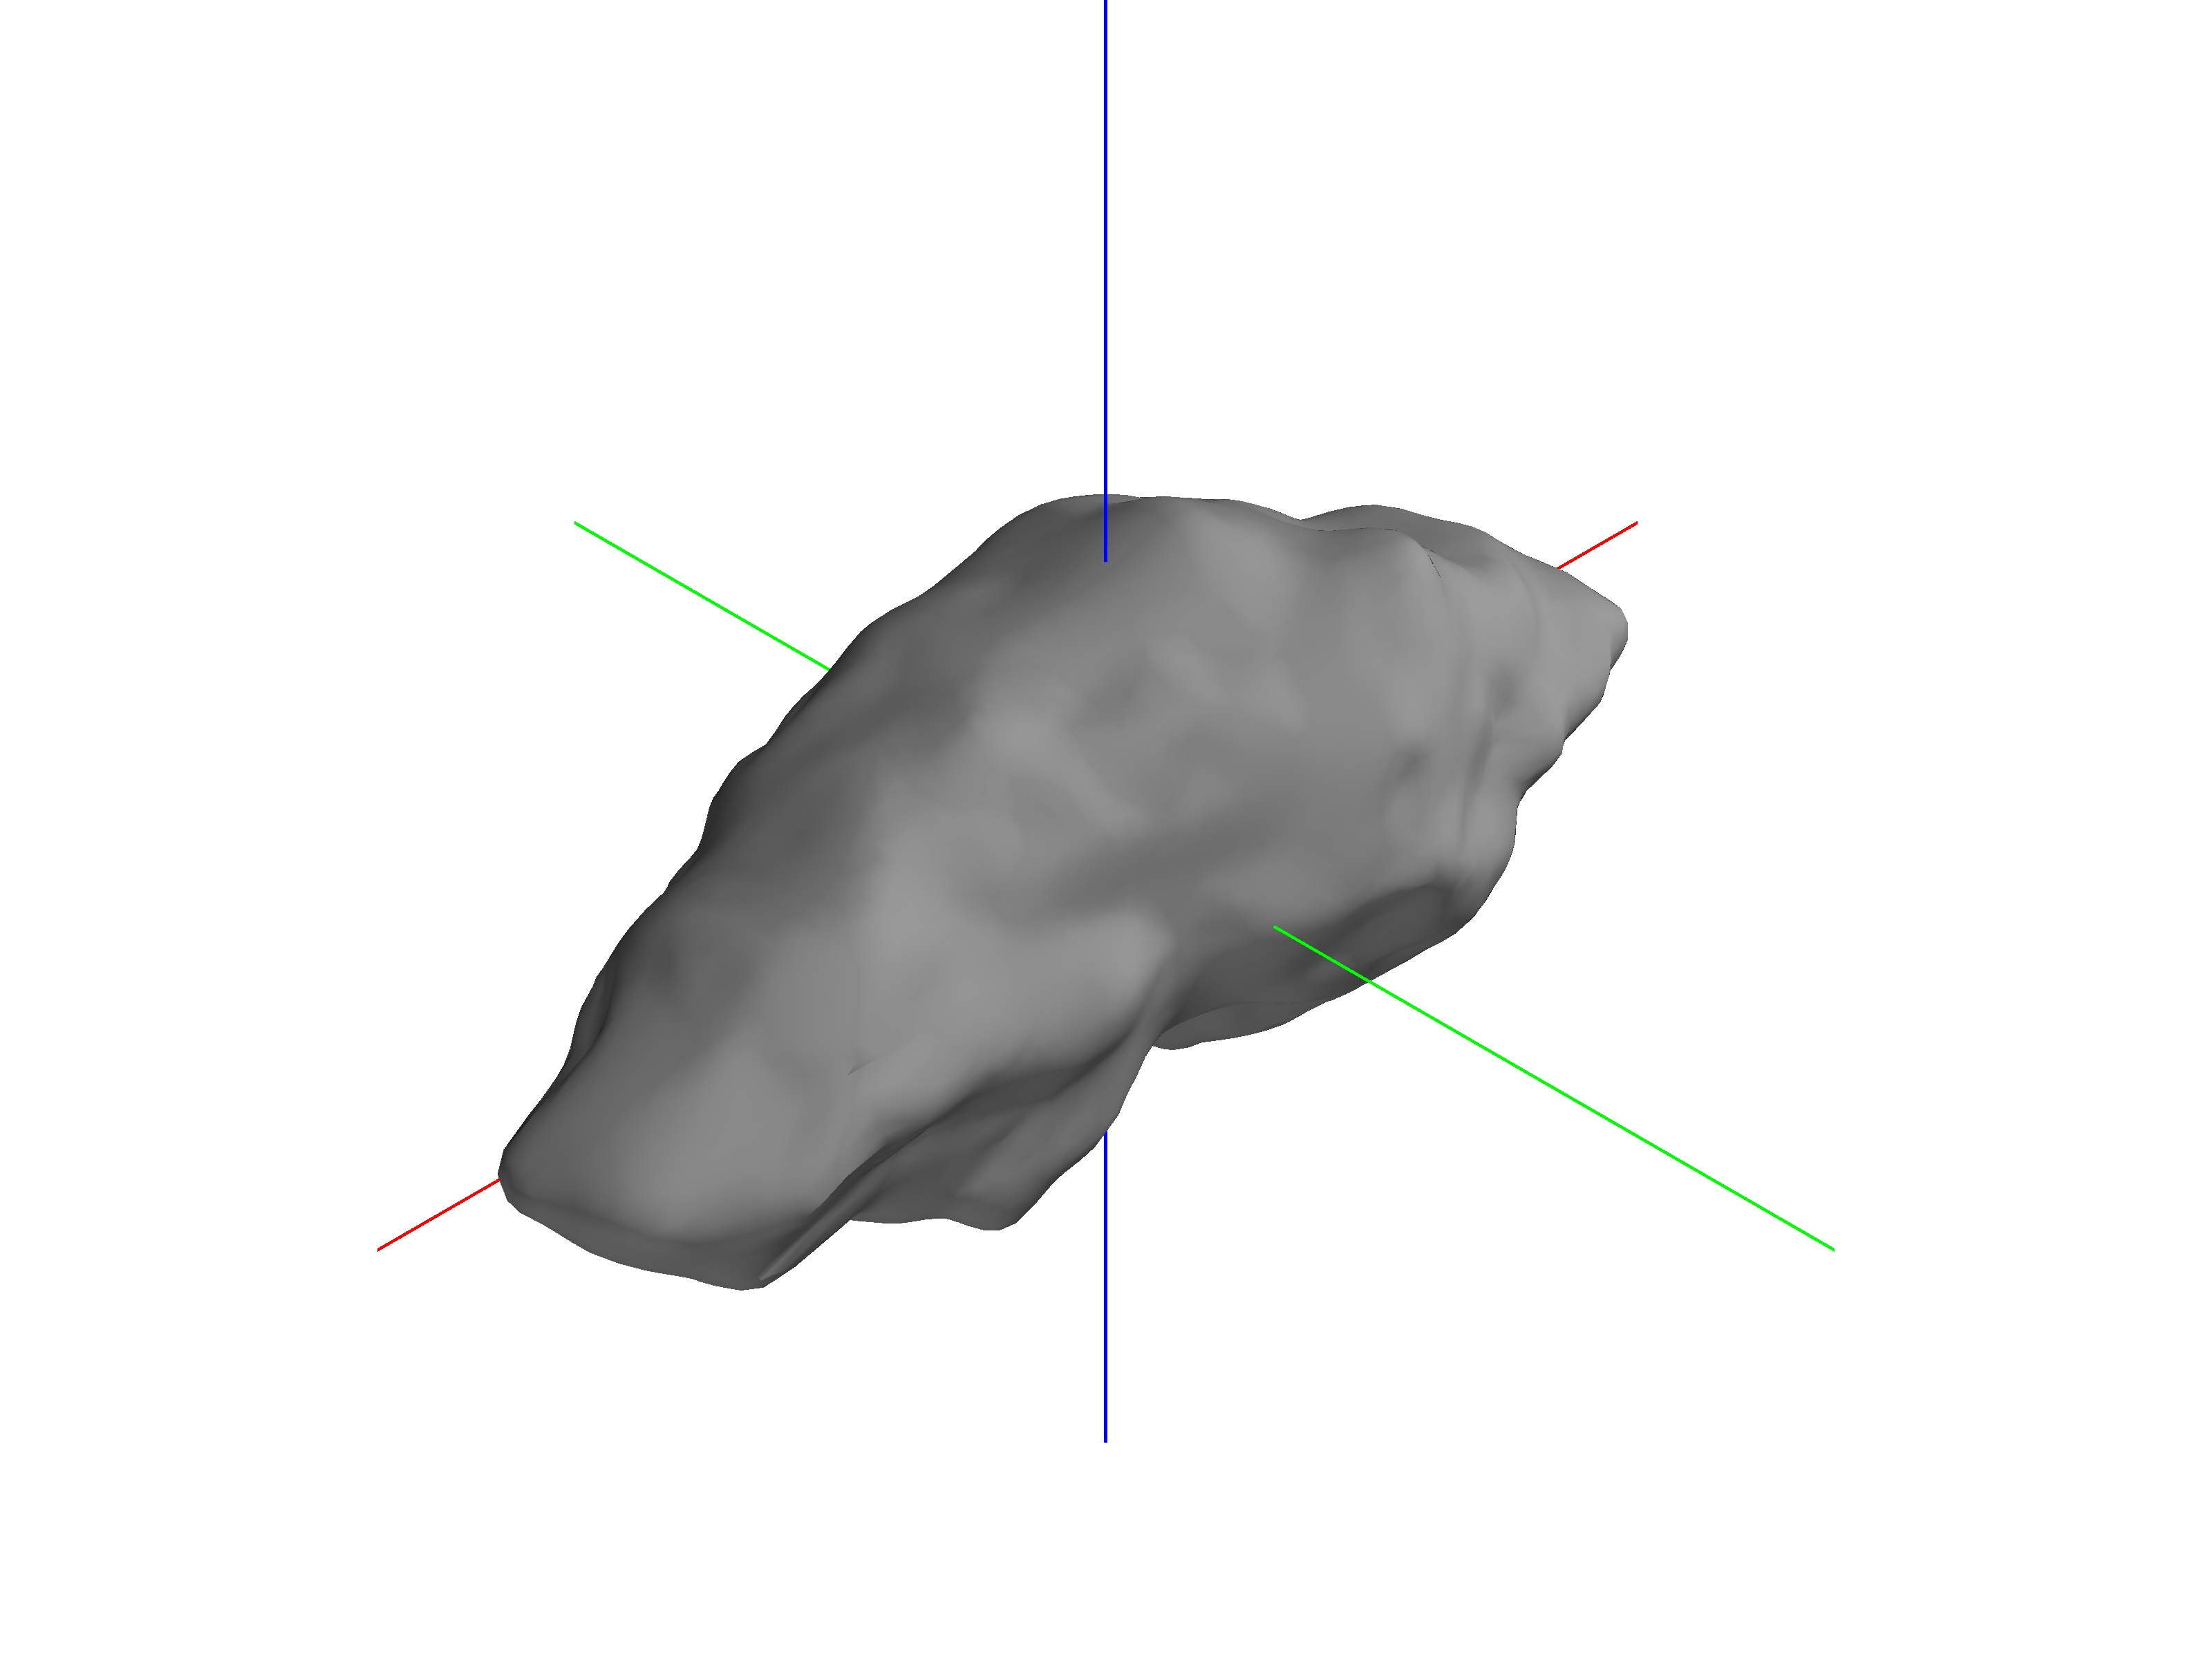
\includegraphics[trim={20cm 15cm 20cm 15cm},clip,keepaspectratio,width=0.5\textwidth]{figures/computational_geometry/mesh_update/geographos/partial_7489.jpg}}{VPlayer.swf}%
        \includemedia[
        keepaspectratio,
        activate=pagevisible,
        addresource=videos/geographos_weight.mp4,
        flashvars={source=videos/geographos_weight.mp4}
        ]{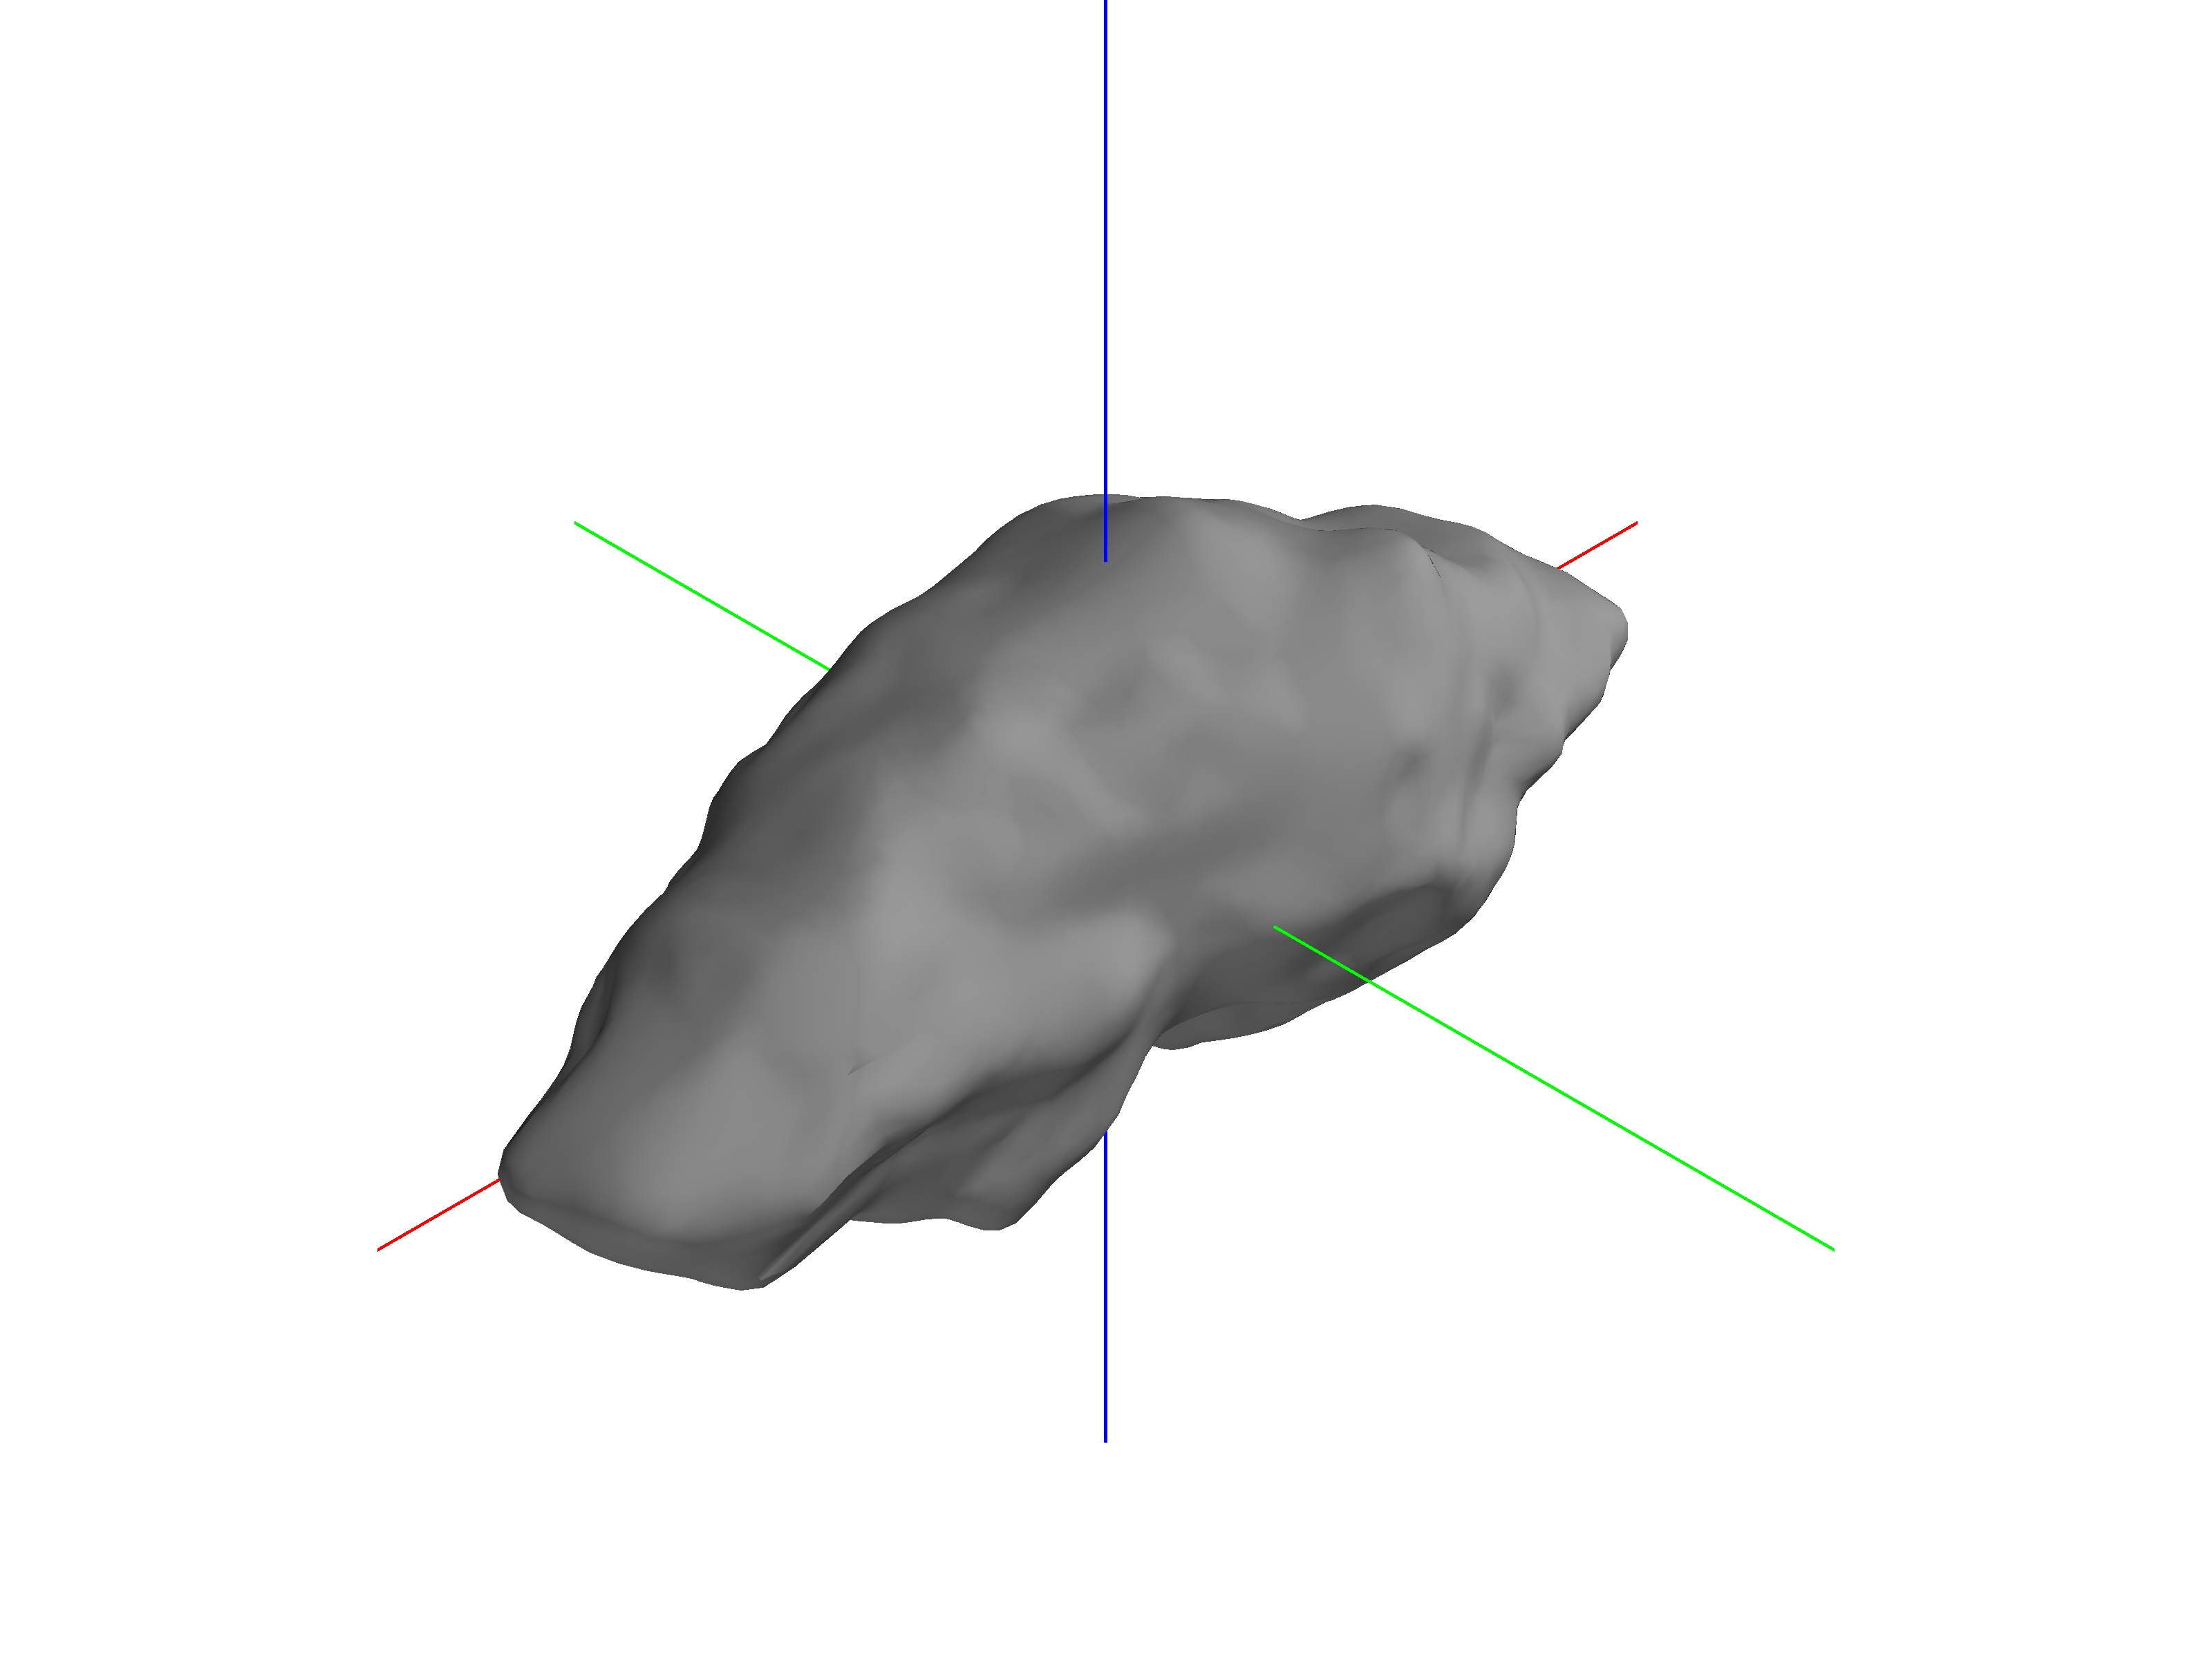
\includegraphics[trim={20cm 15cm 20cm 15cm},clip,keepaspectratio,width=0.5\textwidth]{figures/computational_geometry/mesh_update/geographos/partial_7489.jpg}}{VPlayer.swf}
\end{center}
\end{frame}

\begin{frame}{Golevka Reconstruction}
    \begin{itemize}
        \item Potentially hazardous Apollo group asteroid discovered in 1995
    \end{itemize}
    \begin{center}
        \includemedia[
        keepaspectratio,
        activate=pagevisible,
        addresource=videos/golevka.mp4,
        flashvars={source=videos/golevka.mp4}
        ]{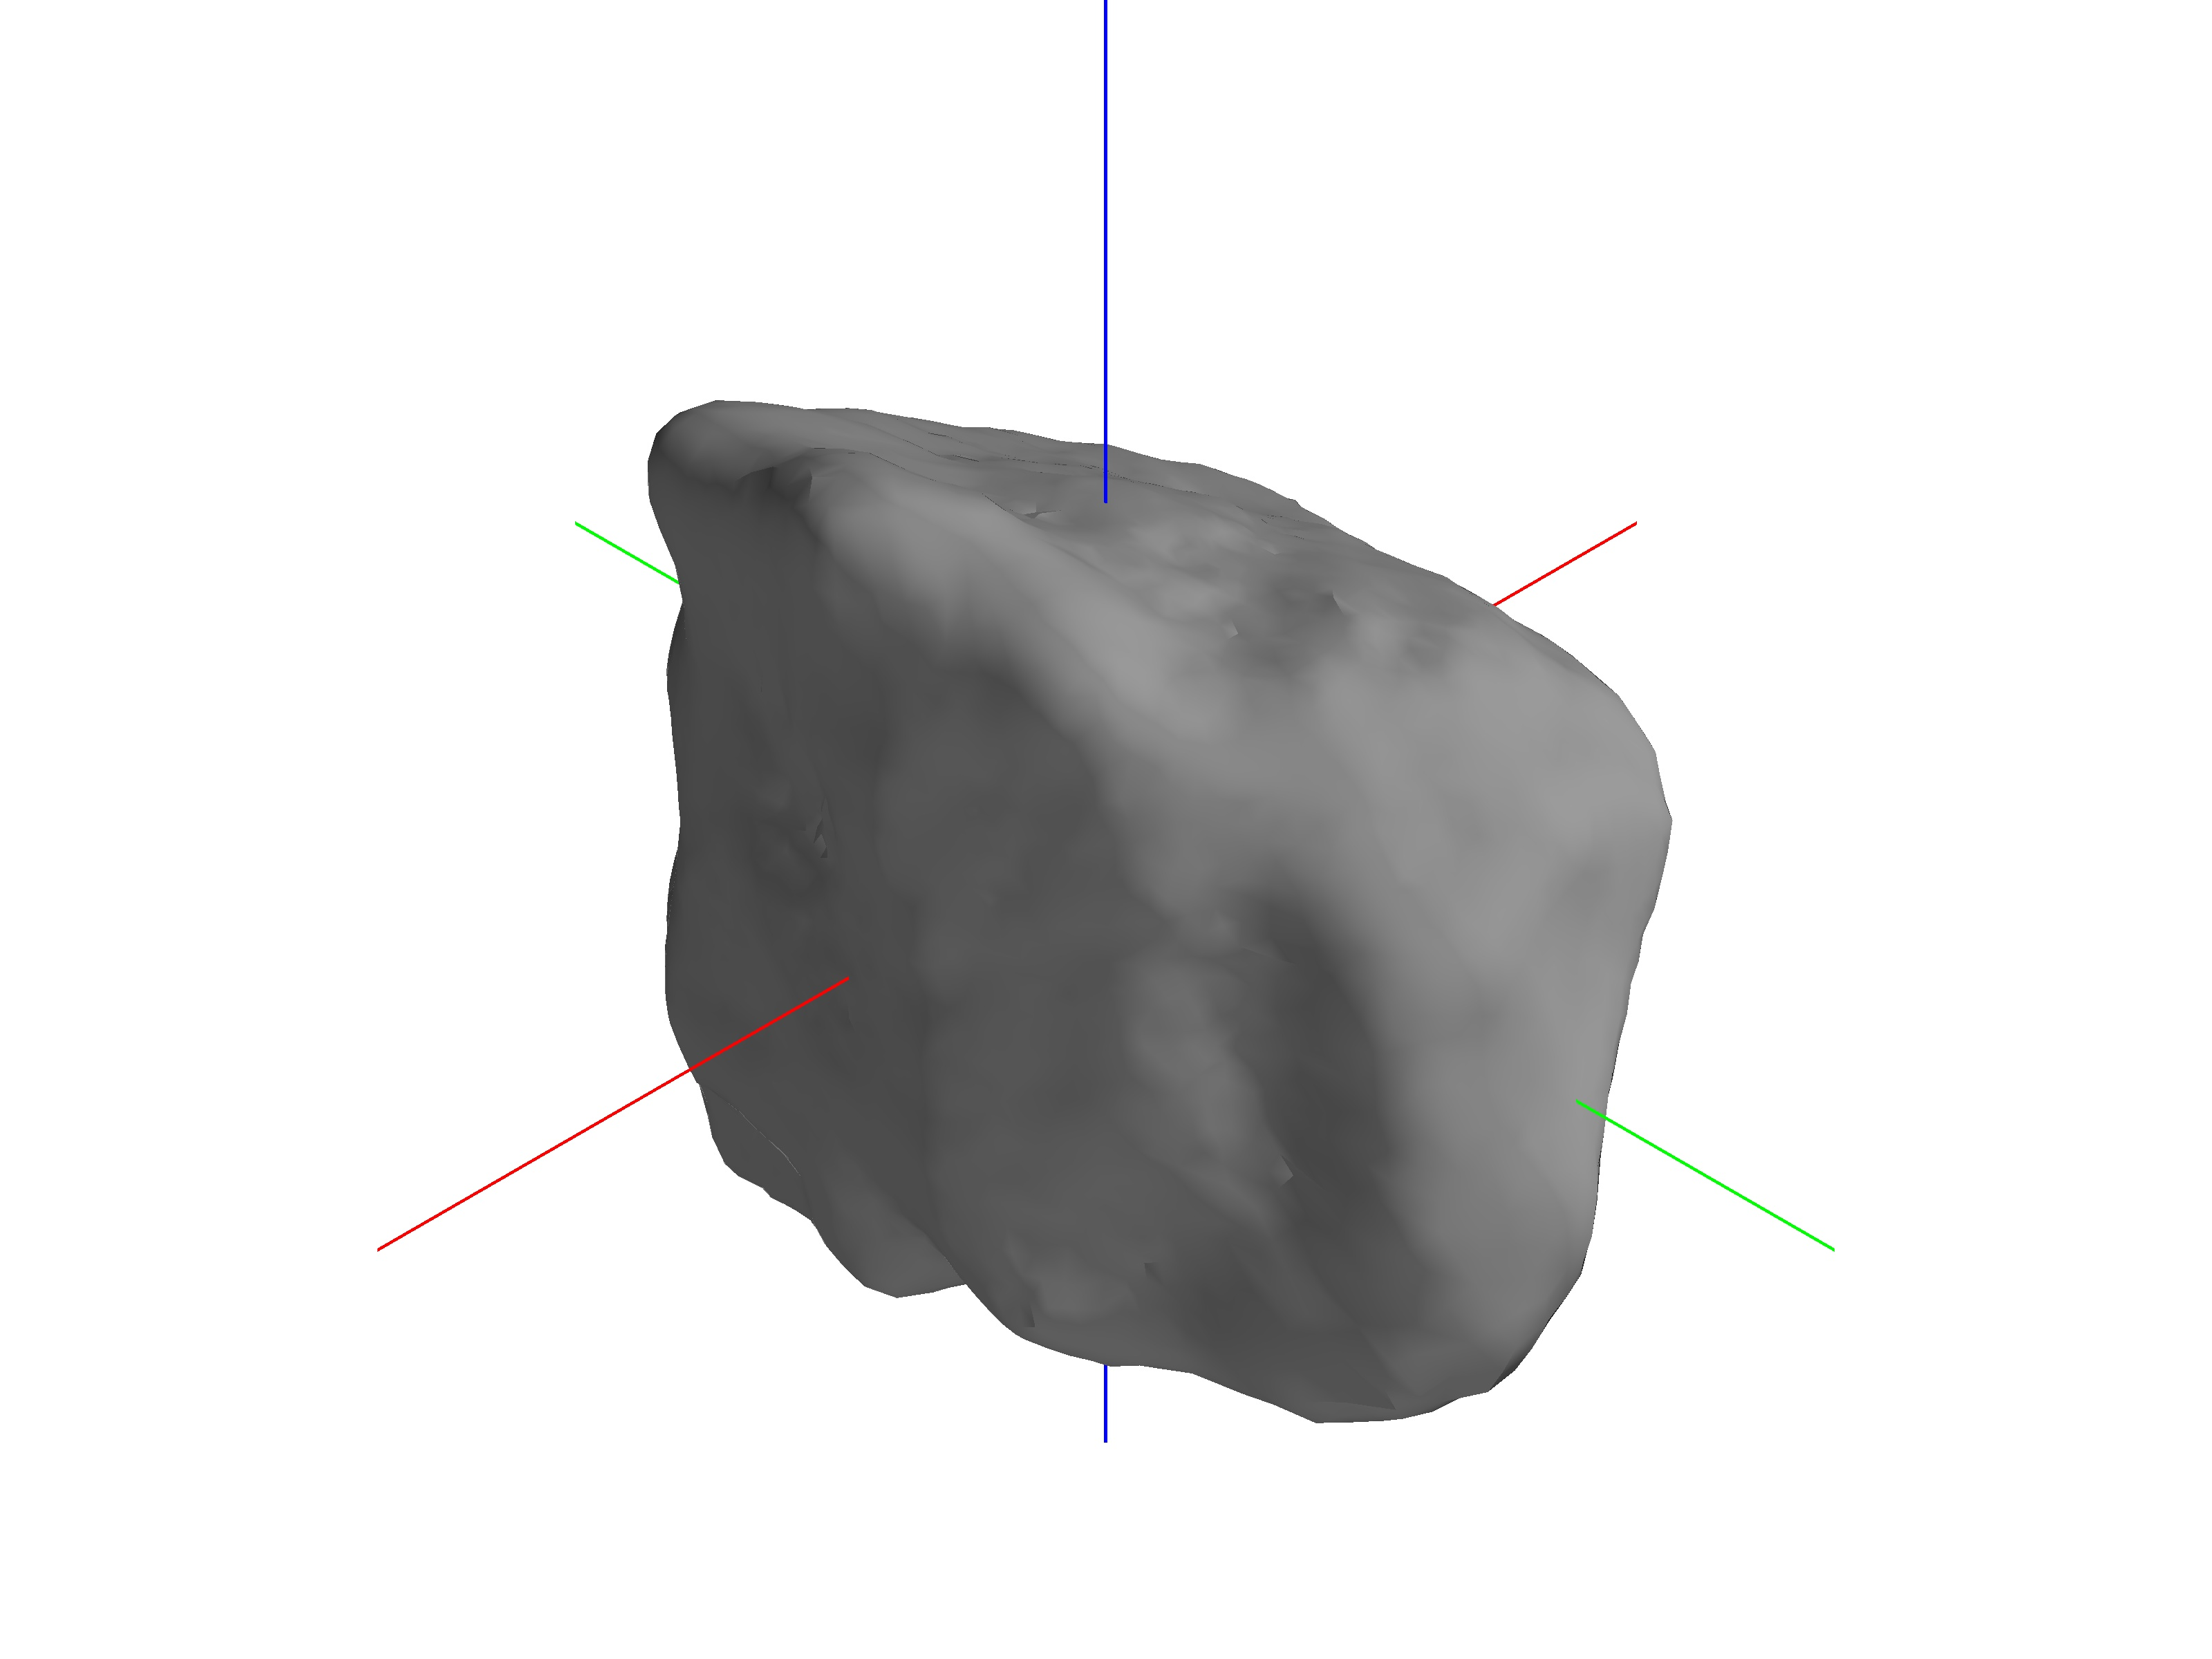
\includegraphics[trim={20cm 10cm 20cm 10cm},clip,keepaspectratio,width=0.5\textwidth]{figures/computational_geometry/mesh_update/golevka/partial_5285.jpg}}{VPlayer.swf}%
        \includemedia[
        keepaspectratio,
        activate=pagevisible,
        addresource=videos/golevka_weight.mp4,
        flashvars={source=videos/golevka_weight.mp4}
        ]{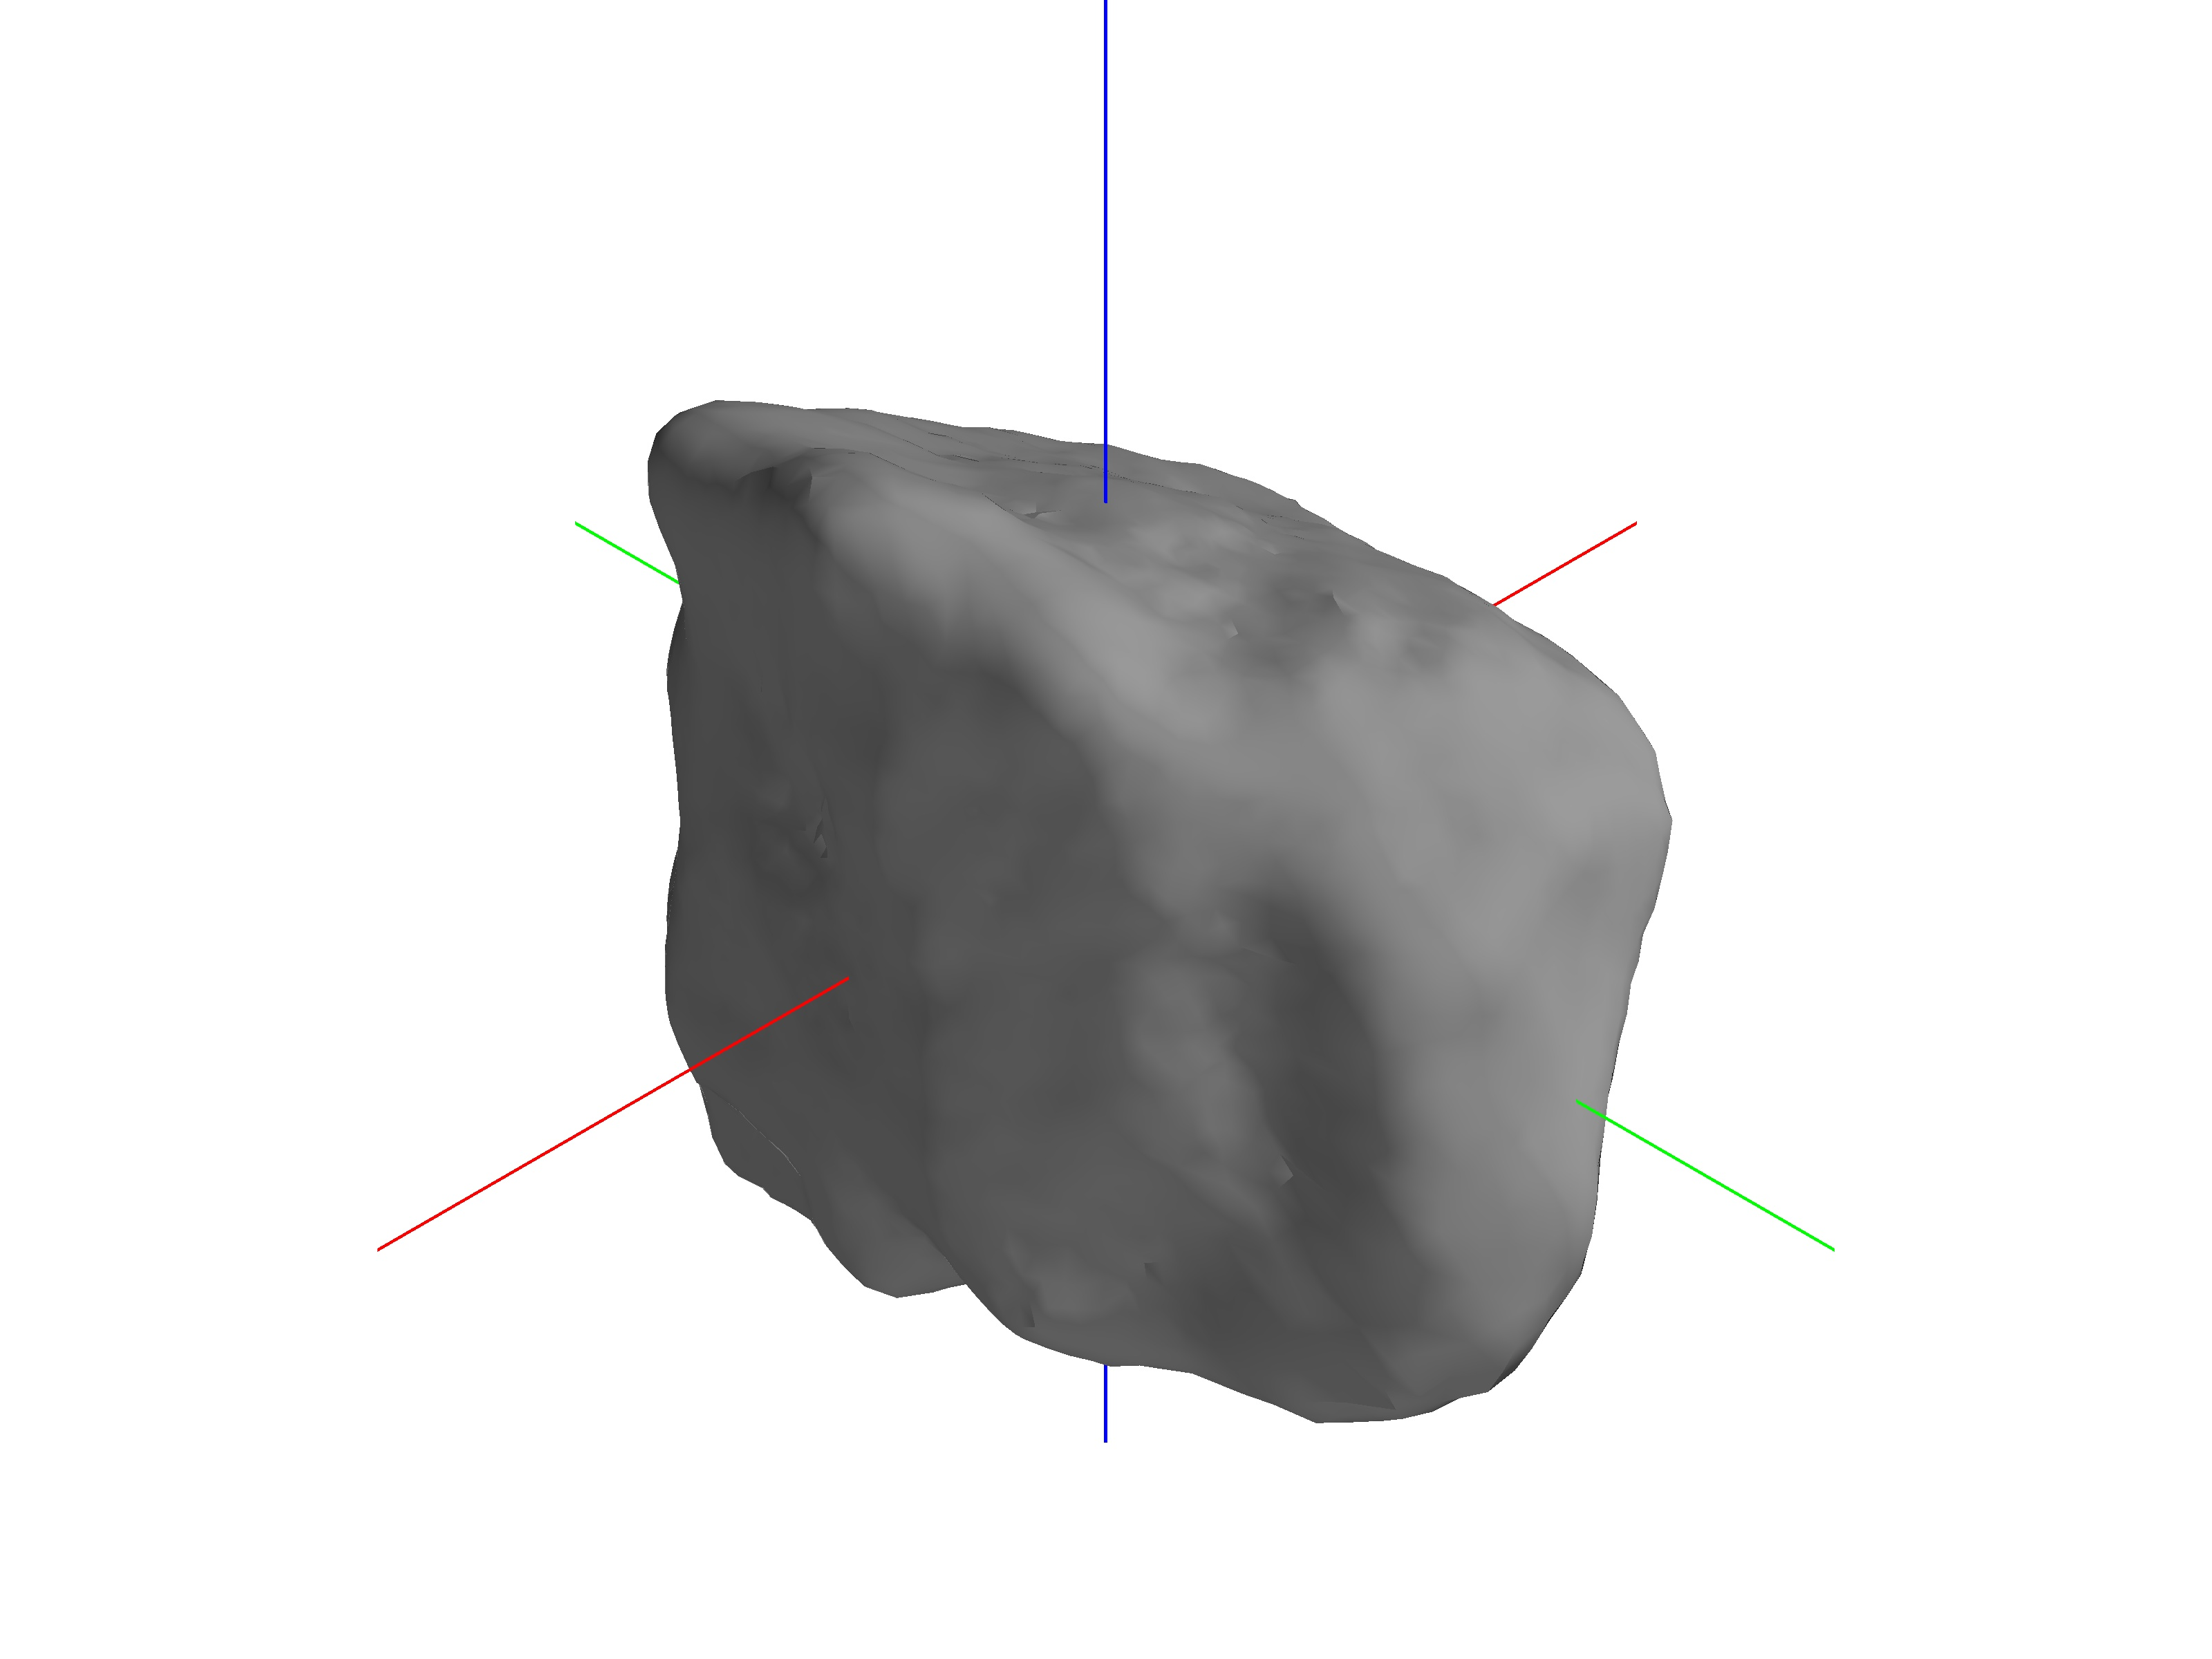
\includegraphics[trim={20cm 10cm 20cm 10cm},clip,keepaspectratio,width=0.5\textwidth]{figures/computational_geometry/mesh_update/golevka/partial_5285.jpg}}{VPlayer.swf}
\end{center}
\end{frame}

\subsection{Guidance}
\begin{frame}{Optimal Guidance}
    \begin{itemize}
        \item Cost function used to determine future states which provides best measurements
        \item User selected weighting between: uncertainty, distance, and control effort
            \begin{align*}
                J_i (\ipos, \iatt, \aatt) = \alpha_w J_{w_i} + \alpha_d J_{d_i}(\rpos) + \alpha_c J_{c_i}(\rpos)
            \end{align*}
    \end{itemize}

    52760 exploration videos
\end{frame}

\subsection{Refinement}
\begin{frame}{Landing Site Selection}
    \begin{itemize}
        \item The shape estimate provides sufficient detail to determine the surface slope
            \begin{align*}
                \cos \parenth{ \pi - \phi } = \frac{\vc{n}_f \cdot U_m}{\norm{U_m}},
            \end{align*}
        \item The desired landing area selected to minimize: slope and distance
        \item Desired landing area used for multi-resolution refinement
    \end{itemize}
    \begin{center}
        \only<1>{
        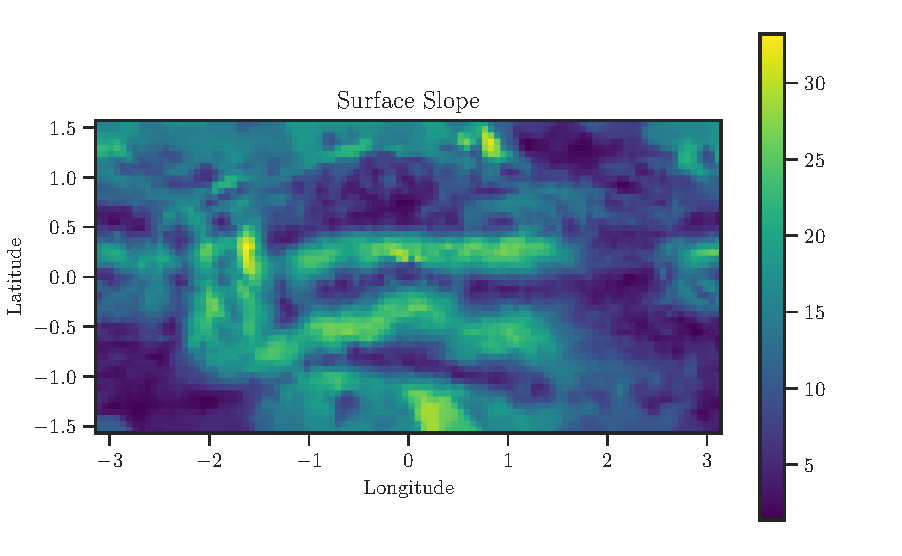
\includegraphics[width=0.5\textwidth]{figures/computational_geometry/dynamic_exploration/castalia/refine/slope.pdf}%
        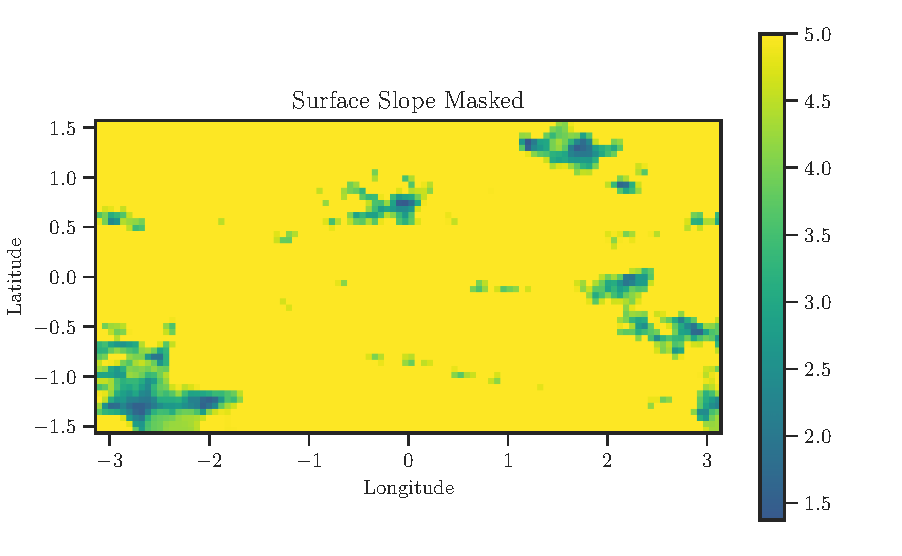
\includegraphics[width=0.5\textwidth,keepaspectratio]{figures/computational_geometry/dynamic_exploration/castalia/refine/slope_masked.pdf}
    }
    \only<2>{
        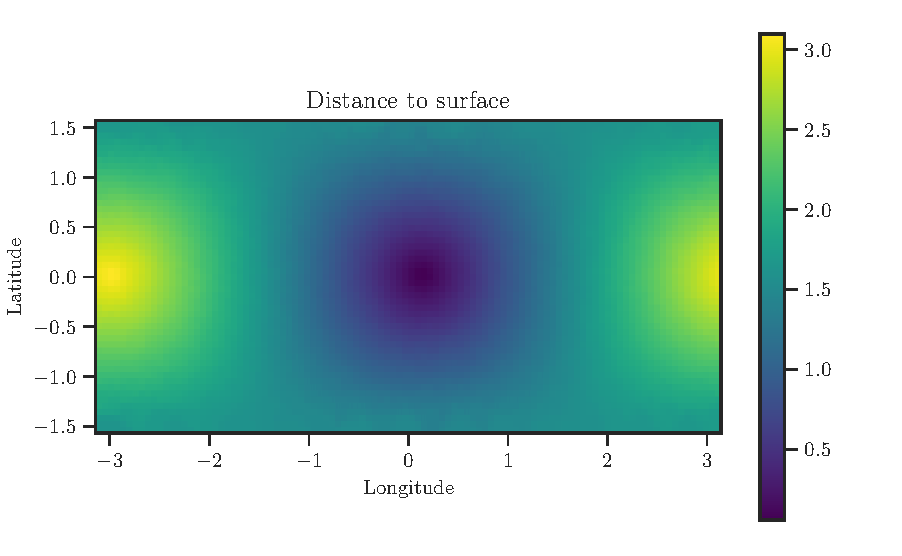
\includegraphics[width=0.5\textwidth]{figures/computational_geometry/dynamic_exploration/castalia/refine/dist.pdf}%
        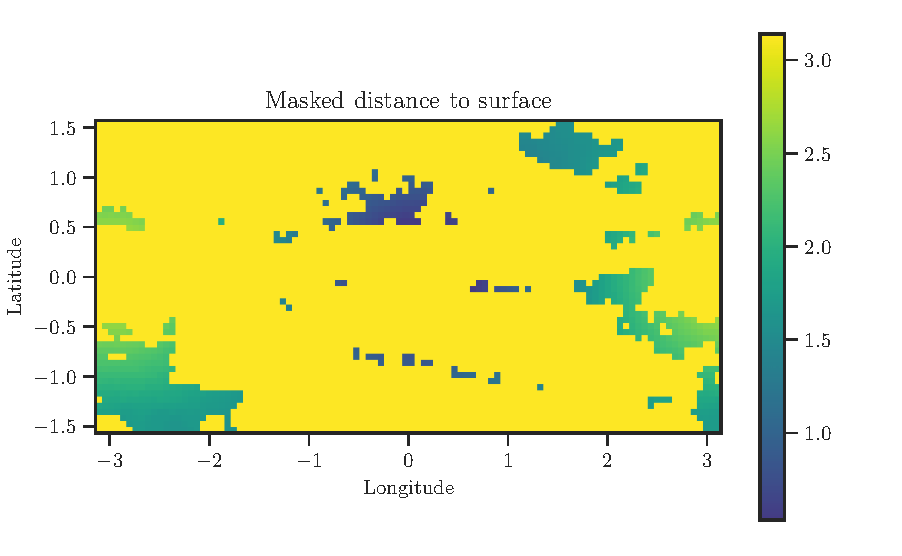
\includegraphics[width=0.5\textwidth,keepaspectratio]{figures/computational_geometry/dynamic_exploration/castalia/refine/dist_masked.pdf}
    }
    \only<3>{
        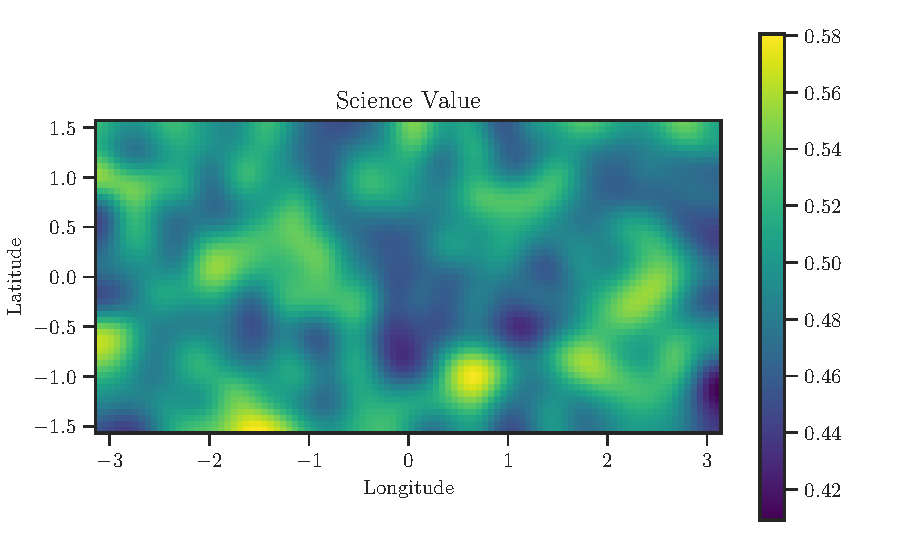
\includegraphics[width=0.5\textwidth]{figures/computational_geometry/dynamic_exploration/castalia/refine/science.pdf}%
        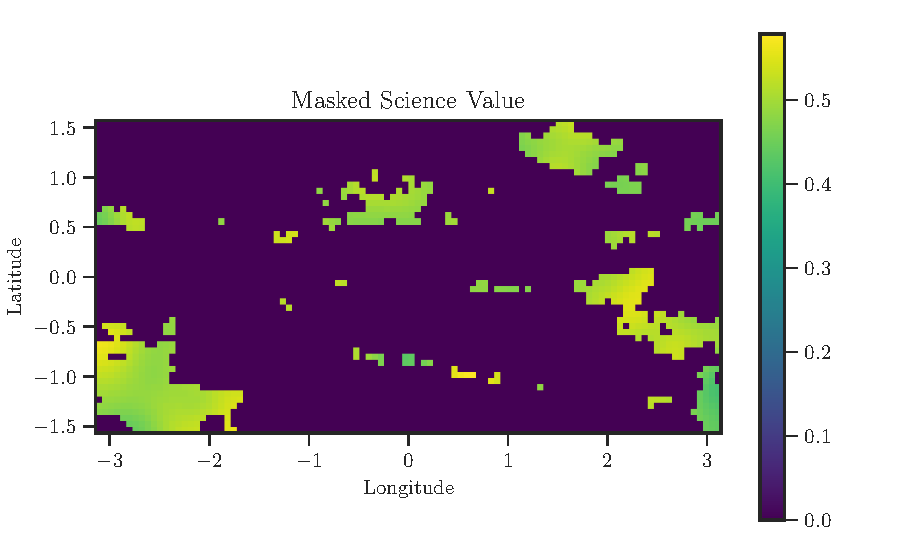
\includegraphics[width=0.5\textwidth,keepaspectratio]{figures/computational_geometry/dynamic_exploration/castalia/refine/science_masked.pdf}
    }
    \only<4>{
        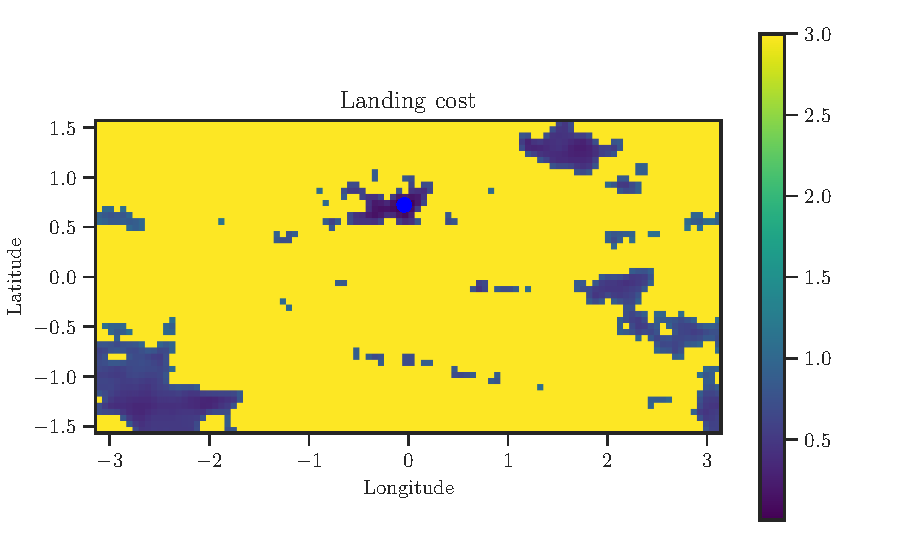
\includegraphics[width=0.5\textwidth]{figures/computational_geometry/dynamic_exploration/castalia/refine/cost.pdf}%
    }
    \end{center}
\end{frame}

\begin{frame}{Multi-resolution refinement}
    \begin{itemize}
        \item The mesh resolution limits the size of captured features
        \item A uniform high resolution mesh would be computationally intractable
    \end{itemize}
    \begin{center}%
        
\includegraphics[width=0.49\textwidth]{figures/computational_geometry/isotropic/original_cube.jpg}%
        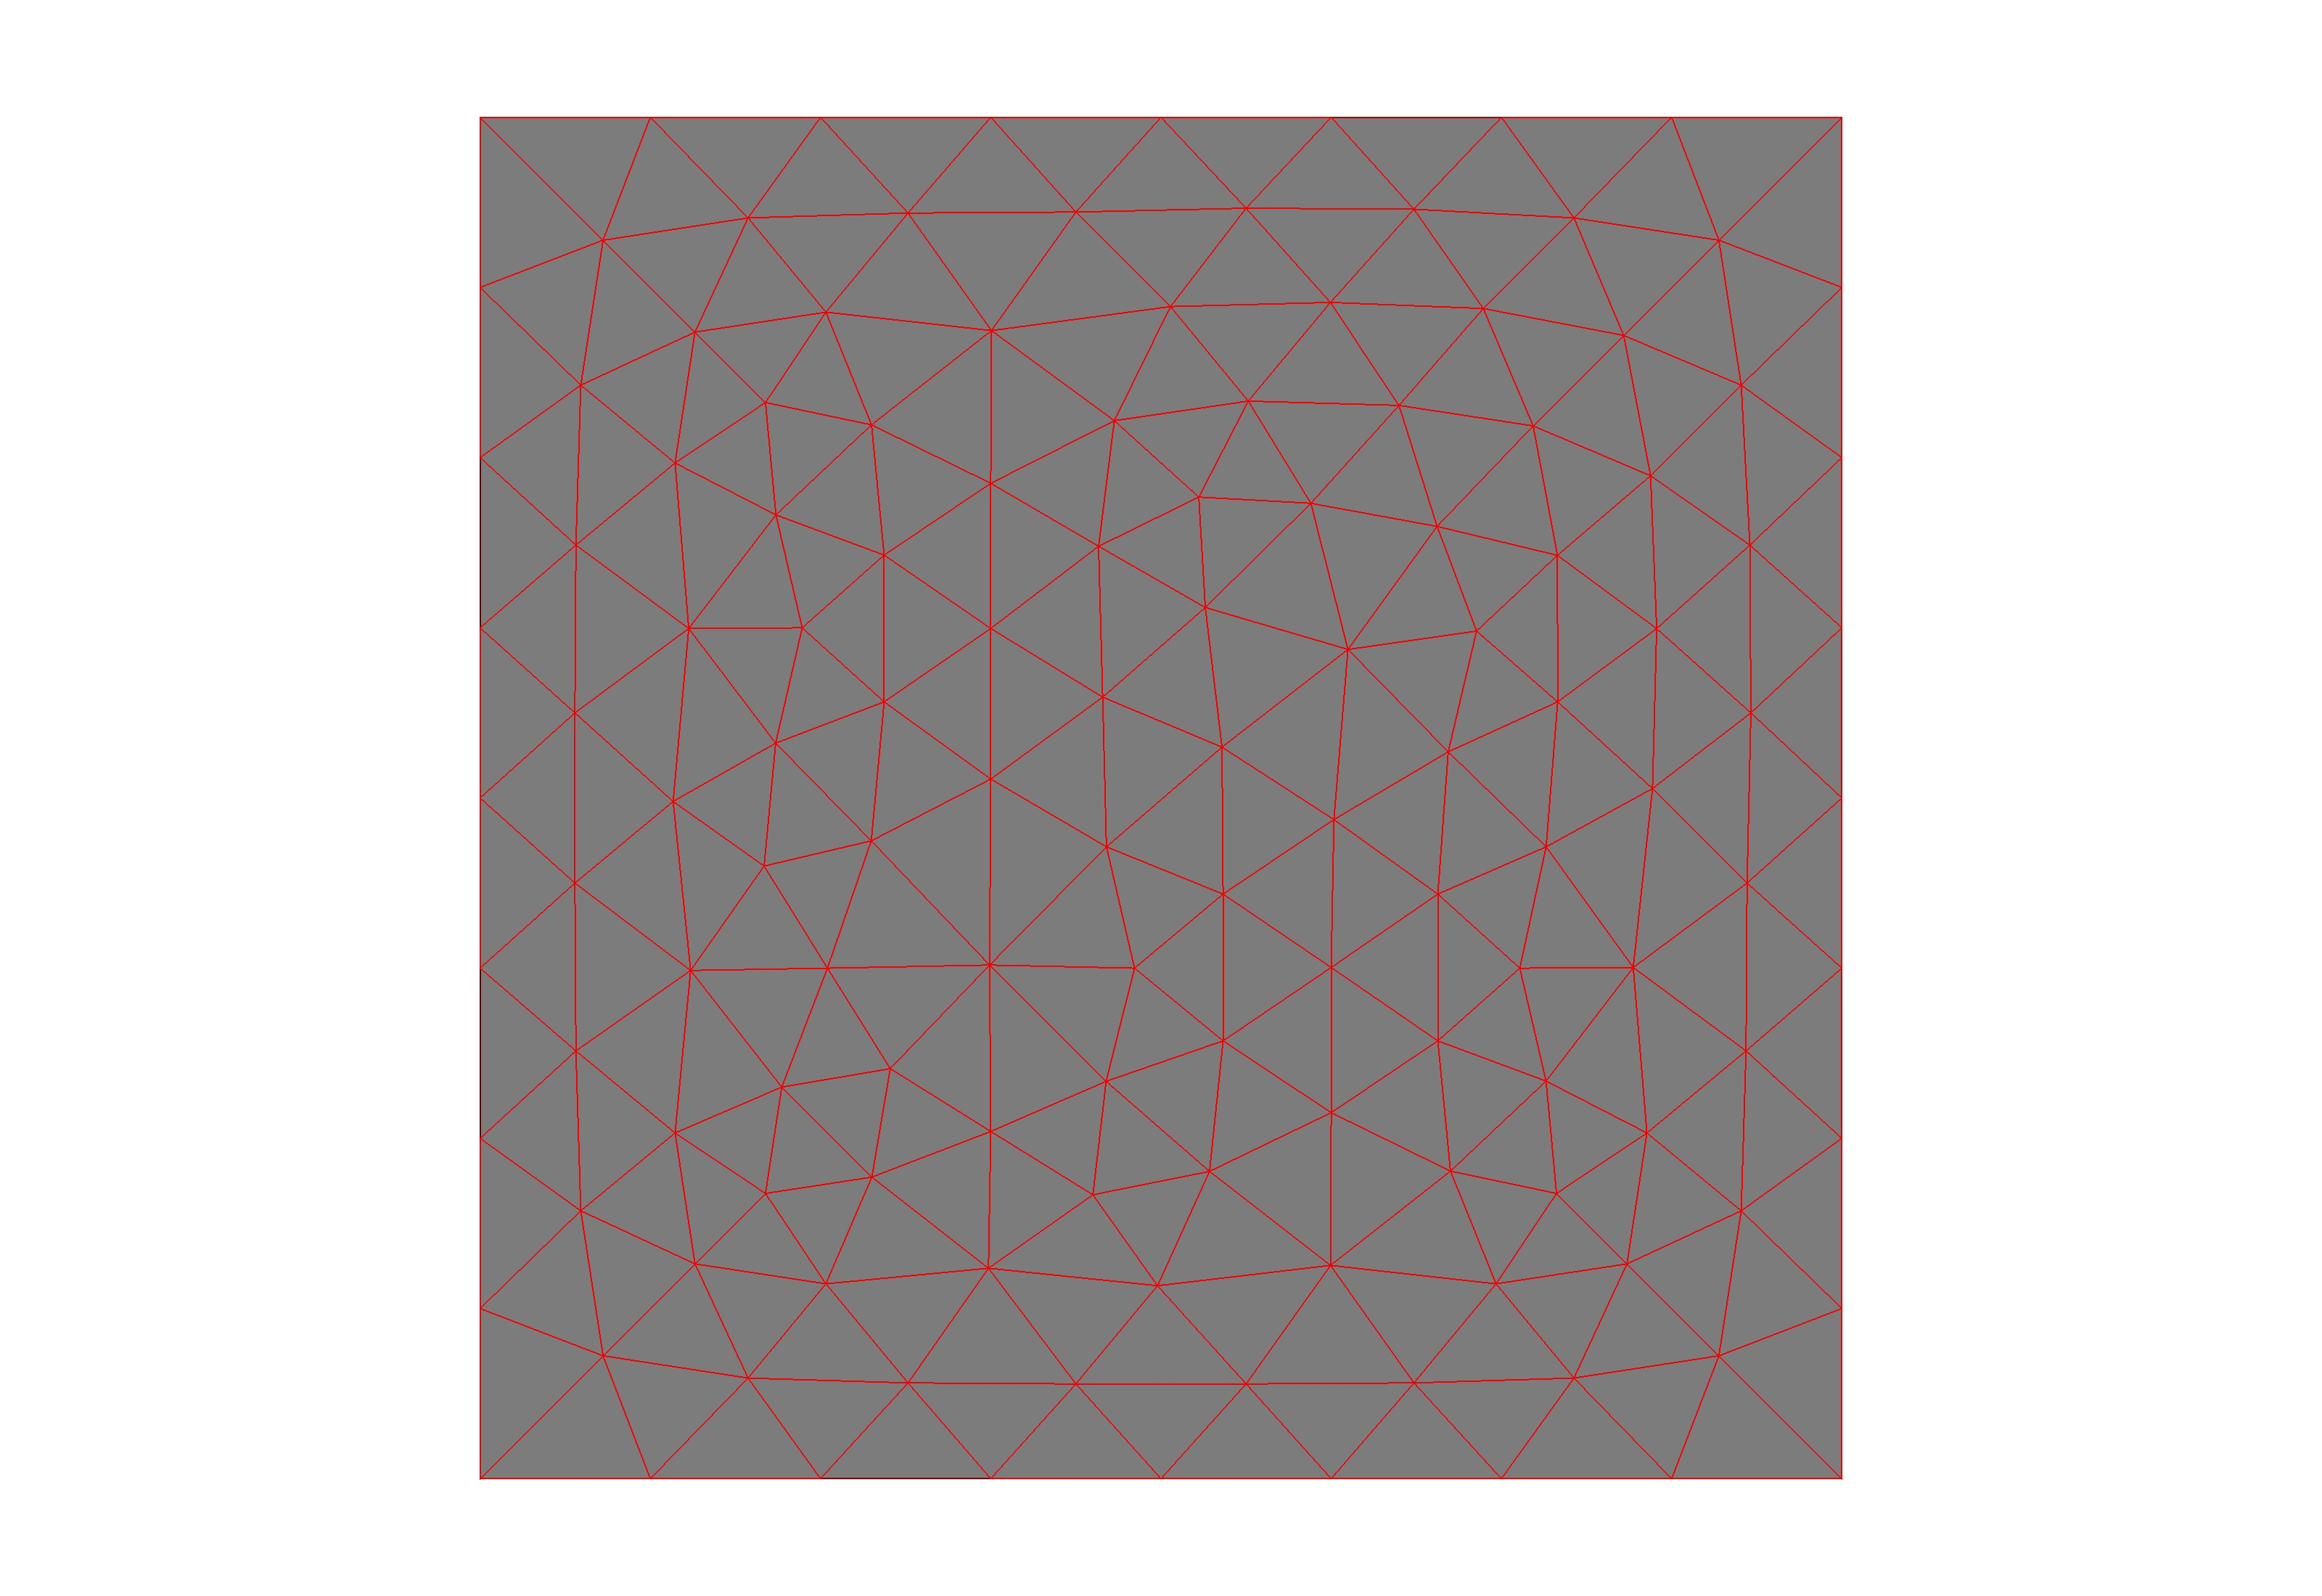
\includegraphics[width=0.49\textwidth]{figures/computational_geometry/isotropic/remesh_cube.jpg}
    \end{center}
\end{frame}

\begin{frame}{4769 Castalia exploration and landing}
    \begin{center}
        Show exploration, refinement and landing videos
    \end{center}
\end{frame}

